%%%%%%%%%%%%%%%%%%%%%%%%%%%%%%%%%%%%%%%%%
% kaobook
% LaTeX Template
% Version 1.0 (2/2/19)
%
% This template originates from:
% https://www.LaTeXTemplates.com
%
% Authors:
% Federico Marotta (federicomarotta@mail.com)
% Based on the doctoral thesis of Ken Arroyo Ohori (https://3d.bk.tudelft.nl/ken/en)
% and on the Tufte-LaTeX class.
% Modified for LaTeX Templates by Vel (vel@latextemplates.com)
%
% License:
% GPL Version 3 (see included LICENSE file)
%
%%%%%%%%%%%%%%%%%%%%%%%%%%%%%%%%%%%%%%%%%

%----------------------------------------------------------------------------------------
%	PACKAGES AND OTHER DOCUMENT CONFIGURATIONS
%----------------------------------------------------------------------------------------

\documentclass[
	fontsize=10pt, % Base font size
	twoside=true, % Use different layouts for even and odd pages (in particular, if twoside=true, the margin column will be always on the outside)
	%open=any, % If twoside=true, uncomment this to force new chapters to start on any page, not only on right pages
	%chapterprefix=true, % Uncomment to use the word "Chapter" before chapter numbers everywhere they appear
	%chapterentrydots=true, % Uncomment to output dots from the chapter name to the page number in the table of contents
	numbers=noenddot, % Comment to output dots after chapter numbers; the most common values for this option are: enddot, noenddot and auto (see the KOMAScript documentation for an in-depth explanation)
	%draft=true, % If uncommented, images will be replaced by empty boxes
	%overfullrule=true, % If uncommented, overly long lines will be marked by a black box
]{kaobook}

% Load common packages and commands
\usepackage{styles/environments}
\usepackage{styles/mdftheorems}
%\usepackage{styles/plaintheorems}

% Load packages for testing
\usepackage{blindtext}
\usepackage{zhlipsum}
%\usepackage{showframe}
%\usepackage{showlabels}

%----------------------------------------------------------------------------------------
%	MY TRACES Stared
%----------------------------------------------------------------------------------------

\usepackage{multirow}
\usepackage{amsmath,bm,amssymb,bbm} % i need to express " $ \to $ "、加粗单字符、数学公式分行、斜平行∥符号(这个本来是要\txfonts包的,但似乎不声明就可以用,应该是哪个包里调用了它了;另外,如果在这里调用了这个包,编译会出错,因为声明了太多数学字体)

% \usepackage{mathrsfs} % 为了使用数学上的 \mathscr 花体
% \DeclareMathAlphabet{\mathscr}{OT1}{pzc}{m}{it}
% \usepackage{amsbsy} % 为了使用 \pmb 懒人加粗法 以加粗 无法被其他命令加粗的 \mathscr,并且用法为 \pmb{\mathscr E}, 其他用法均不行

% \DeclareMathAlphabet{\mathpzc}{OT1}{pzc}{m}{it} % 显示效果与 \mathscr 一样
% \DeclareMathAlphabet{\mathcal}{OT1}{pzc}{m}{it} % 显示效果与 \mathscr 一样

% \usepackage{boondox-cal} % 三者均使用 \mathbcal、\mathcal 生成粗、细花体;较斜但花,效果类似 \mathscr
\usepackage{boondox-calo} % 三者均使用 \mathbcal、\mathcal 生成粗、细花体;较正但花
% \usepackage{dutchcal} % 三者均使用 \mathbcal、\mathcal 生成粗、细花体;正且不花,但即使粗也很细。 但由于 \mathbcal M 所生成的花体M太像小m,我就放弃了这种字体; 但该字体确实很好看,很舍不得放弃它。

% \usepackage{titling} 我需要使用 \thank 命令 以代替 \footnote 命令(有冲突,不能使用)
% \thanksmarkseries{arabic} % 更改标记模式为数字

\usepackage{extarrows}

\renewcommand{\thefootnote}{\Roman{footnote}} % 修改 \footnotemark 和 \footnote 中 \footnotemark 部位的 编号
% 不想使用默认的 \fnsymbol{footnote} 即 *, +、#、§ , ¶, k, ? ?, **, # 的形式作为脚注, 可以把脚注改为符号上标, 宏包 footmisc 提供了自定义符号的命令。
% 在任何 math 环境中使用 footnote 命令,均会出现2个、4个相同的脚注, 因此改用 \footnotemark 和 \footnotetext 命令。 并且 \footnotemark 与 \footnotetext 不能挨在一起, 得分开, 否则也会出现重复注释 ———— 应该是 \footnotetext 不能放在 split 环境 中; 并且 第一个 \footnotetext 最好出现在 equation 环境内, 否则注释的横线距离公式有多余间隔。
\renewcommand{\thempfootnote}{\Roman{mpfootnote}} % 盒子环境中的 \footnotetext 的编号 默认是 a,b,c, 现改为 I,II,III

%----------------------------------------------------------------------------------------
%	MY TRACES Ended
%----------------------------------------------------------------------------------------

\graphicspath{{images/}{./}} % Paths in which to look for images

\addbibresource{main.bib} % Bibliography file

\makeindex[columns=3, title=按字母排序的索引, intoc] % Create an index

\makeglossaries % Create a glossary

\makenomenclature % Create nomenclature

%----------------------------------------------------------------------------------------
\renewcommand\proofname{证明}
\begin{document}

%----------------------------------------------------------------------------------------
%	BOOK INFORMATION
%----------------------------------------------------------------------------------------

\titlehead{\texttt{ETP} Company}
\subject{一场发生在脑海深处的自发极化}

\title[What is Light?]{What is Light? \\ Try hard to {\normalfont\texttt{Understand \&\ Expand}} it}
\subtitle{A General Description of Light}

\author[尘归尘]{尘归尘 \thanks{A \LaTeX\ lover}}

\date{\today}

\publishers{闵可夫斯基\ 出版社}

%----------------------------------------------------------------------------------------

\frontmatter % Denotes the start of the pre-document content, uses roman numerals

%----------------------------------------------------------------------------------------
%	OPENING PAGE
%----------------------------------------------------------------------------------------

% \makeatletter
% \extratitle{
	% 	% In the title page, the title is vspaced by 9.5\baselineskip
	% 	\vspace*{9\baselineskip}
% 	\vspace*{\parskip}
% 	\begin{center}
% 		% In the title page, \huge is set after the komafont for title
% 		\usekomafont{title}\huge\@title
% 	\end{center}
% }
% \makeatother

%----------------------------------------------------------------------------------------
%	COPYRIGHT PAGE
%----------------------------------------------------------------------------------------

\makeatletter
\uppertitleback{\@titlehead} % Header

\lowertitleback{
	\textbf{Disclaimer}\\
	你可以编辑这个页面来满足你的需要。例如,这里有一个无版权的声明、一个版权页标记和其他一些信息。这一页是基于肯·阿罗约·奥赫里的论文的相应页面,改动很小。
	
	\medskip
	
	\textbf{No copyright}\\
	\cczero\ This book is released into the public domain using the CC0 code. To the extent possible under law, I waive all copyright and related or neighbouring rights to this work.
	
	To view a copy of the CC0 code, visit: \\\url{http://creativecommons.org/publicdomain/zero/1.0/}
	
	\medskip
	
	\textbf{Colophon} \\
	This document was typeset with the help of \href{https://sourceforge.net/projects/koma-script/}{\KOMAScript} and \href{ttps://www.latex-project.org/}{\LaTeX} using the \href{https://github.com/fmarotta/kaobook/}{kaobook} class.
	
	The source code of this book is available at:\\\url{https://github.com/fmarotta/kaobook}
	
	(You are welcome to contribute!)
	
	\medskip
	
	\textbf{Publisher} \\
	First printed in Jan 2019 by \@publishers
}
\renewcommand{\maketag@@@}[1]{\hbox{\m@th\normalsize\normalfont#1}} % 强制 \equation 下公式的编号为正常大小 (MY TRACES)
\makeatother

%----------------------------------------------------------------------------------------
%	DEDICATION
%----------------------------------------------------------------------------------------

\dedication{
	世界的和谐体现在形式和数量上,自然哲学的心和灵魂以及一切诗歌都体现在数学美的概念上。\\
	\flushright -- D'Arcy Wentworth Thompson
}

%----------------------------------------------------------------------------------------
%	TITLE PAGE
%----------------------------------------------------------------------------------------

% Note that \maketitle will actually print many pages.
% Based on 上述四部分 BOOK INFORMATION,OPENING PAGE,COPYRIGHT PAGE,DEDICATION 利用 KOM Script automatically 生成的 TIITL PAGE。

% If twoside=false, \uppertitleback and \lowertitleback are not printed. To overcome this issue, we set twoside=semi just before printing the title pages, and set it back to false just after the title pages.
\KOMAoptions{twoside=semi}
\maketitle[3] % The [3] assigns "page 3" to the title, so that the cover page would get "page 1" (see KOMAScript documentation about maketitle)
\KOMAoptions{twoside=false}

%----------------------------------------------------------------------------------------
%	PREFACE
%----------------------------------------------------------------------------------------

\chapter*{前言}
\addcontentsline{toc}{chapter}{前言}

我的观点是,每个\LaTeX \xspace 极客,至少在他的一生中有一次,都觉得有必要创建自己的类:这就是发生在我身上的事情,这就是结果,但是,这应该被看作是一个仍在进行中的工作。实际上,这个类并不完全是原创的,但它是我在许多指南、教程、博客和text.stackexchange.com文章中发现的所有最佳思想的混合体。特别是,主要的想法来自两个来源:

\begin{itemize}
	\item \href{https://3d.bk.tudelft.nl/ken/en/}{Ken Arroyo Ohori}'s 
		\href{ttps://3d.bk.tudelft.nl/ken/en/nl/ken/en/2016/04/17/a-1.5-column-layout-in-latex.html}{Doctoral 
			Thesis}, which served, with the author's permission, as a 
		backbone for the implementation of this class;
	\item The 
		\href{https://github.com/Tufte-LaTeX/tufte-latex}{Tufte-Latex 
			Class}, which was a model for the style.
\end{itemize}

本书第一章是导论,涵盖了本课程最基本的特点。接下来,有一堆章节专门讨论所有的命令和环境,你可以用来写一本书;特别地,它将解释如何添加注释、图形和表以及引用。第二部分讨论页面布局和设计,以及其他特性,如彩色框和定理环境。

我开始写这门课是作为一个实验,因此它应该被视为。由于它一直是我个人使用的缩进,它可能不是完美的,但我发现它很满意的用途,我想让它。我分享这篇文章,希望有人能从这里找到写作的灵感。

\begin{flushright}
	\textit{Federico Marotta}
\end{flushright}


%----------------------------------------------------------------------------------------
%	TABLE OF CONTENTS & LIST OF FIGURES/TABLES
%----------------------------------------------------------------------------------------

\begingroup

% Define the style for the TOC, LOF, and LOT
%\setstretch{1}
%\hypersetup{linkcolor=DarkBlue}
\setlength{\textheight}{23cm}

% Turn on compatibility mode for the etoc package
\etocstandarddisplaystyle % "toc display" as if etoc was not loaded
\etocstandardlines % "toc lines as if etoc was not loaded

\tableofcontents % Output the table of contents

\listoffigures % Output the list of figures
% Comment both of the following lines to have the LOF and the LOT on different pages
\let\cleardoublepage\bigskip
\let\clearpage\bigskip

\listoftables % Output the list of tables
\let\cleardoublepage\bigskip
\let\clearpage\bigskip

\listoftheorems

\endgroup

%----------------------------------------------------------------------------------------
%	MAIN BODY
%----------------------------------------------------------------------------------------

\mainmatter % Denotes the start of the main document content, resets page numbering and uses arabic numbers

\setchapterstyle{kao}
\setchapterpreamble[u]{\margintoc}
\chapter{引言}
\labch{intro}

\section{主要思想}

许多现代印刷教科书采用了突出的页边空白处的布局,在这里可以显示小的数字、表格、注释和几乎所有的东西。可以说,这种布局通过将主要文本与辅助材料分离来帮助组织讨论,而辅助材料同时又非常接近文本中引用它的地方。

这份文件的目的并不是要道歉,因为有许多更适合这项任务的作者;所有这些单词的目的只是填充空间,以便读者可以看到用kaobook类编写的书是什么样子的。同时,我还将尝试说明类的特性。

kaobook背后的主要思想来自于这个\href{https://3d.bk.tudelft.nl/ken/en/2016/04/17/a-1.5-column-layout-in latex。html}{blog post},实际上这个类的名称是专门为这篇文章的作者Ken Arroyo Ohori命名的,他允许我根据他的论文创建一个类。因此,如果你想知道更多喜欢1.5栏布局的理由,一定要阅读他的博客文章。

您可能已经注意到,灵感的另一个来源是\href{https://github.com/tuft-latex/tuft-latex}{tuft-latex类}。设计相似的原因是很难改进已经很好的东西。但是,我认为这个类比tuft - latex更灵活。例如,我尝试只使用标准包,并尽可能少地从头实现;\sidenote{这也意味着更容易理解和贡献类开发。实际上,还有很多地方需要改进,所以如果您感兴趣,可以在github上查看存储库!}因此,只要您阅读了提供该特性的包的文档,定制任何东西都应该非常容易。

在本书中,我将阐述该类的主要特性,并提供有关如何使用和更改内容的信息。让我们开始吧。

\section{本类的功能}
\labsec{does}

\Class{kaobook}类更关注文档结构,而不是样式。实际上,众所周知的\LaTeX\xspace 原则是结构和样式应该尽可能地分离(参见\vrefsec{does})。这意味着这个类将只提供命令、环境和一般情况下的机会来执行用户可能使用或不使用的操作。实际上,类中嵌入了一些样式问题,但是用户可以轻松地定制它们。

主要特点如下:

\begin{description}
	\item[Page Layout] 减少文本宽度是为了提高可读性,并为页边距留出空间,以便显示任何类型的元素。
	\item[Chapter Headings] 相对于tuft-latex,我们提供了多种章节标题可供选择;例子将在后面的章节中看到。
	\item[Page Headers] 它们跨越整个页面,包括页边距,并在双侧模式下交替显示章节和节名。\sidenote[-2mm][]{这是Tufte设计的另一个不同之处。}
	\item[Matters] The commands \Command{frontmatter}, 
	\Command{mainmatter} and \Command{backmatter} have been redefined in 
	order to have automatically wide margins in the main matter, and 
	narrow margins in the front and back matters. However, the page 
	style can be changed at any moment, even in the middle of the 
	document.
	\item[Margin text] We provide commands \Command{sidenote} and 
	\Command{marginnote} to put text in the 
	margins.\sidenote[-2mm][]{Sidenotes (like this!) are numbered while 
	marginnotes are not}
	\item[Margin figs/tabs] A couple of useful environments is 
	\Environment{marginfigure} and \Environment{margintable}, which, not 
	surprisingly, allow you to put figures and tables in the margins 
	(\cfr \reffig{marginmonalisa}).
	\item[Margin toc] Finally, since we have wide margins, why don't add 
	a little table of contents in them? See \Command{margintoc} for 
	that.
	\item[Hyperref] \Package{hyperref} is loaded and by default we try 
	to add bookmarks in a sensible way; in particular, the bookmarks 
	levels are automatically reset at \Command{appendix} and 
	\Command{backmatter}. Moreover, we also provide a small package to 
	ease the hyperreferencing of other parts of the text.
	\item[Bibliography] We want the reader to be able to know what has 
	been cited without having to go to the end of the document every 
	time, so citations go in the margins as well as at the end, as in 
	Tufte-Latex. Unlike that class, however, you are free to customise 
	the citations as you wish.
\end{description}

\begin{marginfigure}[-5.5cm]
	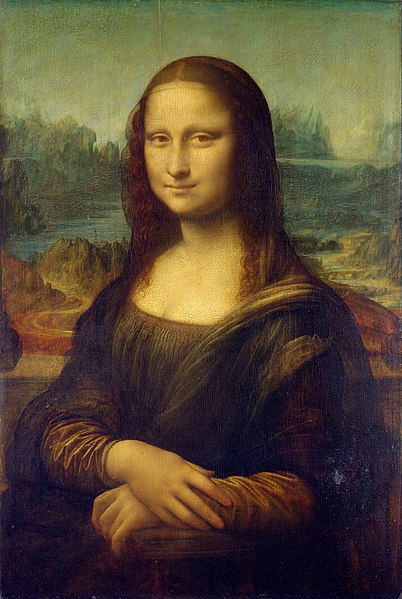
\includegraphics{monalisa}
	\caption[The Mona Lisa]{The Mona Lisa.\\ 
	\url{https://commons.wikimedia.org/wiki/File:Mona_Lisa,_by_Leonardo_da_Vinci,_from_C2RMF_retouched.jpg}}
	\labfig{marginmonalisa}
\end{marginfigure}

The order of the title pages, table of contents and preface can be 
easily changed, as in aly \LaTeX\ document. In addition, the class is 
based on \KOMAScript's \Class{scrbook}, therefore it inherits all the 
goodies of that.

\section{本类未实现的功能}
\labsec{doesnot}

As anticipated, further customisation of the book is left to the user. 
Indeed, every book may have sidenotes, margin figures and so on, but 
each book will have its own fonts, toc style, special environments and 
so on. For this reason, in addition to the class, we provide only 
sensible defaults, but if these features are not nedded, they can be 
left out. These special packages are located in the \Path{style} 
directory, which is organised as follows:

\begin{description}
	\item[style.sty] 这个包包含页面布局、页眉和页脚、章节标题和整个文档中使用的字体的规范。
	\item[packages.sty] 加载额外的包,用特殊的内容来装饰写作(例如,这里加载\Package{listing}包,因为不是每本书都需要它)。还定义了一些有用的命令,用于以相同的方式打印相同的单词,例如斜体的拉丁单词或逐字的\Package{packages}。
	\item[references.sty] 一些有用的命令来管理标签和引用,再次确保以一致的方式引用相同的元素。
	\item[environments.sty] 提供特殊的环境,比如框。简单和复杂的环境都是可用的;所谓复杂,我们的意思是它们被赋予一个计数器,浮动的,可以放在一个特殊的目录中。\sidenote[-2mm][]{参考 
	\vrefch{mathematics}来获取更多示例。}
	\item[theorems.sty] The style of mathematical environments. 
	Acutally, there are two such packages: one is for plain theorems, 
	\ie the theorems are printed in plain text; the other uses 
	\Package{mdframed} to draw a box around theorems. You can plug the 
	most appropriate style into its document.
\end{description}

\marginnote[2mm]{The audacious users might feel tempted to edit some of 
these packages. I'd be immensely happy if they sent me examples of what 
they have been able to do!}

In the rest of the book, I shall assume that the reader is not a novice 
in the use of \LaTeX, and refer to the documentation of the packages 
used in this class for things that are already explained there. 
Moreover, I assume that the reader is willing to make minor edits to the 
provided packages for styles, environments and commands, if he or she 
does not like the default settings.


\pagelayout{wide} % No margins
\addpart{类选项、命令和环境}
\pagelayout{margin} % Restore margins

\input{chapters/chapter2.tex}
\setchapterpreamble[u]{\margintoc}
\chapter{Margin stuff}

侧记是所有1.5列布局书籍的一个显著特征。事实上,宽边意味着一些材料可以在那里展示。我们对所有的东西都使用边距:旁注、边注、小目录、引文,为什么不呢?,特殊的盒子和环境。

\section{Sidenotes}

Sidenotes are like footnotes, except that they go in the margin, where 
they are more readable. To insert a sidenote, just use the command 
\Command{sidenote\{Text of the note\}}. You can specify a 
mark\sidenote[O]{This sidenote has a special mark, a big O!} with \\ 
\Command{sidenote[mark]\{Text\}}, but you can also specify an offset, 
which moves the sidenote upwards or downwards, so that the full syntax is:

\begin{lstlisting}[style=kaolstplain]
\sidenote[offset][mark]{Text}
\end{lstlisting}

If you use an offset, you always have to add the 
brackets for the mark, but they can be empty.\sidenote{If you want to 
know more about the usage of the \Command{sidenote} command, read the 
documentation of the \Package{snotez} package.} The format of the actual 
sidenote can be changed with the command \Command{setsidenotes}, which 
allows you to modify, for instance, the format of the markers and the 
separator between the marker and the text of the sidenote.

There was an alternative package, \Package{sidenotes}, which we could 
have used. In the end we went for \Package{snotez} because it was the 
one used in Ken Ohori's thesis, which inspired this class. The features 
are very similar, but one additional thing offered by \Package{snotez} 
is that the offset can be specified as a multiple of 
\Command{baselineskip}. For example, if you want to enter a sidenote 
with the normal mark and move it upwards one line, type:

\begin{lstlisting}[style=kaolstplain]
\sidenote[*-1][]{Text of the sidenote.}
\end{lstlisting}

Sidenotes are handled through the \Package{snotez} package, which in 
turn relies on the \Package{marginnote} package.

\section{Marginnotes}

This command is very similar to the previous one. You can create a 
marginnote with \Command{marginnote[offset]\{Text\}}, where the offset 
argument can be left out, or it can be a multiple of 
\Command{baselineskip},\marginnote[-1cm]{While the command for margin 
notes comes from the \Package{marginnote} package, it has been redefined 
in order to change the position of the optional offset argument, which 
now precedes the text of the note, whereas in the original version it 
was at the end. We have also added the possibility to use a multiple of 
\Command{baselineskip} as offset. These things were made only to make 
everything more consistent, so that you have to remember less things!} 
\eg

\begin{lstlisting}[style=kaolstplain]
\marginnote[-12pt]{Text} or \marginnote[*-3]{Text}
\end{lstlisting}

\begin{kaobox}[frametitle=To Do]
A small thing that needs to be done is to renew the \Command{sidenote} 
command so that it takes only one optional argument, the offset. The 
special mark argument can go somewhere else. In other words, we want the 
syntax of \Command{sidenote} to resemble that of \Command{marginnote}.
\end{kaobox}

We load the packages \Package{marginnote}, \Package{marginfix} and 
\Package{placeins}. Since \Package{snotez} uses \Package{marginnote}, 
what we said for marginnotes is also valid for sidenotes. Side- and 
margin- notes are shifted slightly upwards 
(\Command{renewcommand\{\textbackslash marginnotevadjust\}\{3pt\}}) in 
order to allineate them to the bottom of the line of text where the note 
is issued.

\section{Footnotes}

Even though they are not displayed in the margin, we will discuss about 
footnotes here, since sidenotes are mainly intended to be a replacement 
of them. Footnotes force the reader to constantly move from one area of 
the page to the other. Arguably, marginnotes solve this issue, so you 
should not use footnotes. Nevertheless, for completeness, we have left 
the standard command \Command{footnote}, just in case you want to put a 
footnote once in a while.\footnote{And this is how they look like. 
Notice that in the PDF file there is a back reference to the text; 
pretty cool, uh?}

\section{Margintoc}

Since we are talking about margins, we introduce here the 
\Command{margintoc} command, which allows one to put small table of 
contents in the margin. Like other commands we have discussed, 
\Command{margintoc} accepts a parameter for the vertical offset, like 
so: \Command{margintoc[offset]}.

The command can be used in any point of the document, but we think it 
makes sense to use it just at the beginning of chapters or parts. In 
this document I make use of a \KOMAScript\xspace feature and put it in 
the chapter preamble, with the following code:

\marginnote{The font used in the margintoc is the same as the one for 
	the chapter entries in the main table of contents at the beginning 
	of the document.}

\begin{lstlisting}[style=kaolstplain]
\setchapterpreamble[u]{\margintoc}
\chapter{Chapter title}
\end{lstlisting}

Not only textual stuff can be displayed in the margin, but also figures. 
Those will be the focus of the next chapter.

\setchapterimage[6.5cm]{seaside}
\setchapterpreamble[u]{\margintoc}
\chapter[Figures and Tables]{Figures and Tables\footnotemark[0]}

\footnotetext{The credits for the image above the chapter title go to:
	Bushra Feroz --- Own work, CC~BY-SA~4.0, 
	\url{https://commons.wikimedia.org/w/index.php?curid=68724647}}

\section{Normal figures and tables}

可以像插入任何标准\LaTeX\xspace 文档一样插入数字和表。\Package{graphicx}包已经加载并配置好了,其图形宽度等于textwidth,并且调整了高度以保持原始的纵横比。正如您所想象的,标题将被很好地放置在页边空白处。这是在\Package{floatrow}包的帮助下实现的。

这里有一张蒙娜丽莎的照片(\reffig{normalmonalisa})作为例子。标题格式为页边距和边注;如果您想更改标题的某些内容,可以使用\Package{title}包中的命令\ command {captsetup}。请记住,如果您想引用一个图形,标签必须在标题\emph{之后}出现!

\begin{figure}[hb]
	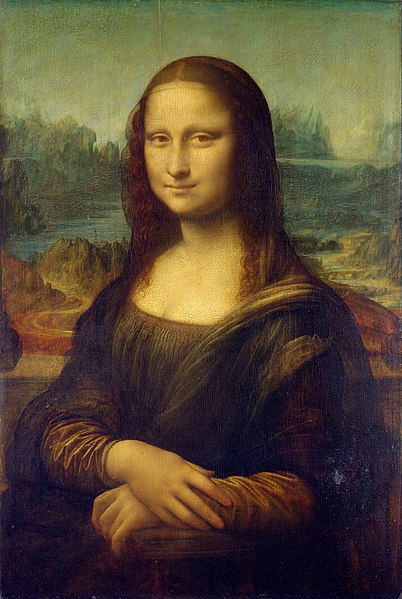
\includegraphics[width=0.45\textwidth]{monalisa}
	\caption[Mona Lisa, again]{It's Mona Lisa again. \blindtext}
	\labfig{normalmonalisa}
\end{figure}

虽然标题的格式由\Package{title}管理,但是它的位置由\Package{floatrow}包处理。取得这样的成绩是很辛苦的,但现在我很满意。在双面模式下,标题以正确的页边距打印。

插入表格和插入数字一样容易,如下面的代码所示:

\begin{lstlisting}
\begin{table}
\begin{tabular}{ c c c c }
	\toprule
	col1 & col2 & col3 & col 4 \\
	\midrule
	\multirow{3}{4em}{Multiple row} & cell2 & cell3 & cell4\\ &
	cell5 & cell6 & cell7 \\ &
	cell8 & cell9 & cell10 \\
	\multirow{3}{4em}{Multiple row} & cell2 & cell3 & cell4 \\ &
	cell5 & cell6 & cell7 \\ &
	cell8 & cell9 & cell10 \\
	\bottomrule
\end{tabular}
\end{table}
\end{lstlisting}

which results in the useless \vreftab{useless}.

\begin{table}[h]
\caption[A useless table]{A useless table.}
\labtab{useless}
\begin{tabular}{ c c c c }
	\toprule
	col1 & col2 & col3 & col 4 \\
	\midrule
	\multirow{3}{4em}{Multiple row} & cell2 & cell3 & cell4\\ &
	cell5 & cell6 & cell7 \\ &
	cell8 & cell9 & cell10 \\
	\multirow{3}{4em}{Multiple row} & cell2 & cell3 & cell4 \\ &
	cell5 & cell6 & cell7 \\ &
	cell8 & cell9 & cell10 \\
	\bottomrule
\end{tabular}
\end{table}

I don't have much else to say, so I will just insert some blind text. 
\blindtext

\section{Margin figures and tables}

可以使用\Environment {marginfigure}环境插入Marginfigures。在这种情况下,整个图片被限制在页边空白处,标题在它下面。\reffig{marginmonalisa}是这样得到的:

\begin{lstlisting}
\begin{marginfigure}
	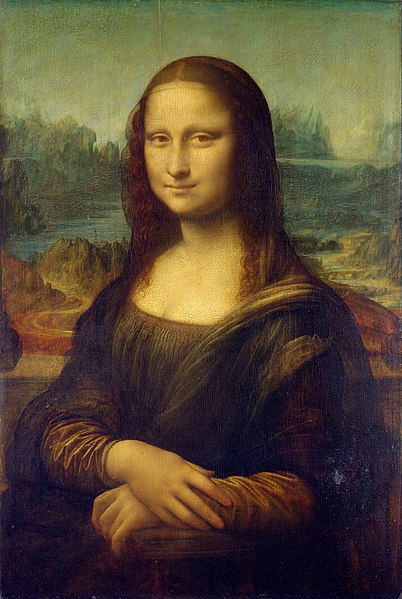
\includegraphics{monalisa}
	\caption[The Mona Lisa]{The Mona Lisa.}
	\labfig{marginmonalisa}
\end{marginfigure}
\end{lstlisting}

There is also the \Environment{margintable} environment, of which 
\reftab{anotheruseless} is an example. Notice how you can place the 
caption above the table by just placing the \Command{caption} command 
before beginning the \Environment{tabular} environment. Usually, figure 
captions are below, while table captions are above. This rule is also 
respected for normal figures and tables: the captions are always on the 
side, but for figure they are aligned to the bottom, while for tables to 
the top.

\begin{margintable}
\caption[Another useless table]{Another useless table.}
\labtab{anotheruseless}
\raggedright
\begin{tabular}{ c c c c }
	\hline
	col1 & col2 & col3 \\
	\hline
	\multirow{3}{4em}{Multiple row} & cell2 & cell3 \\ & cell5 & cell6 
	\\ & cell8 & cell9 \\ \hline
\end{tabular}
\end{margintable}

Marginfigures and tables can be positioned with an optional offset 
command, like so:

\begin{lstlisting}
\begin{marginfigure}[offset]
	\includegraphics{images/seaside}
\end{marginfigure}
\end{lstlisting}

Offset ca be either a measure or a multiple of \Command{baselineskip}, 
much like with \Command{sidenote}, \Command{marginnote} and 
\Command{margintoc}.\todo{Improve this part.} If you are wondering how I 
inserted this orange bubble, have a look at the \Package{todo} package.

\section{Wide figures and tables}

\begin{figure*}[h!]
	\includegraphics{seaside}
	\caption[一个宽阔的海边]{宽阔的海边,宽阔的标题。作品简介:布什拉·费罗兹(Bushra Feroz)著 --- 自己的工作, CC BY-SA 4.0, 
		\url{https://commons.wikimedia.org/w/index.php?curid=68724647}}
\end{figure*}

使用\Environment{figure*}和\Environment{table*}环境,您可以插入跨越整个页面宽度的数字。标题将根据口味被置于下方或上方。

您可能已经注意到了本章开头的全宽图像:但是,它是以一种完全不同的方式设置的,您将在\vrefch{layout}中了解到这一点。现在是处理超引用的时候了。

\setchapterstyle{kao}
%\setchapterpreamble[u]{\margintoc}
\chapter{参考文献}
\labch{references}

\section{引用}

\index{citations}
要引用某人\sidecite{Visscher2008,James2013}非常简单:只需使用\Command{sidecite}\index{\Command{sidecite}}命令。它还没有一个抵消的参数,但它可能会在未来。如您所见,该命令支持多个条目,默认情况下,它在页边空白处打印引用,并将其添加到文档末尾的参考书目中。在这个设置中,我使用了biblatex,但是我认为这是可行的。\sidecite{James2013}注意,这些引用与文本没有任何关系,它们完全是随机的,因为它们只用于说明特性。

要编译包含引用的文档,您需要使用一个外部工具,对于这个类,这个工具是biber。您需要运行以下命令(假设您的tex文件名为main.text):

\begin{lstlisting}[style=kaolstplain]
$ pdflatex main
$ biber main
$ pdflatex main
\end{lstlisting}

\section{术语表和索引}

\index{glossary}
\Class{kaobook}类加载\Package{glossary}和\Package{imakeidx}包,您可以使用它们将词汇表和索引添加到您的图书中。例如,我以前定义了一些术语表条目,现在我将使用它们,如下所示:\gls{computer}。\Package{glossary}还允许您使用缩略词,如下所示:这是完整版\acrfull{fpsLabel},这是简短版\acrshort{fpsLabel}。这些条目将出现在术语表的后面。

Unless you use \href{https://www.overleaf.com}{Overleaf} or some other 
fancy IDE for \LaTeX, you need to run an external command from your 
terminal in order to compile a document with a glossary. In particular, 
the commands required are:\sidenote[-2mm][]{These are the commands you 
would run in a UNIX system; I have no idea on how it works in Windows.}

\begin{lstlisting}[style=kaolstplain]
$ pdflatex main
$ makeglossaries main
$ pdflatex main
\end{lstlisting}

Note that you need not run \texttt{makeglossaries} every time you 
compile your document, but only when you change the glossary entries.

\index{index}
To create an index, you need to insert the command 
\lstinline|\index{subject}| whenever you are talking about 
\enquote{subject} in the text. For instance, at the start of this 
paragraph I would write \lstinline|index{index}|, and an entry would be 
added to the Index in the backmatter. Check it out!

\marginnote[2mm]{In theory, you would need to run an external command 
for the index as well, but luckily the package we suggested, 
	\Package{imakeidx}, can compile the index automatically.}

\index{nomenclature}
A nomenclature is just a special kind of index; you can find one at the end of
this book. To insert a nomenclature, we use the package \Package{nomencl} and
add the terms with the command \Command{nomenclature}. We put then a
\Command{printnomenclature} where we want it to appear.

Also with this package we need to run an external command to compile the 
document, otherwise the nomenclature will not appear:

\begin{lstlisting}[style=kaolstplain]
$ pdflatex main
$ makeindex main.nlo -s nomencl.ist -o main.nls
$ pdflatex main
\end{lstlisting}

These packages are all loaded in 
\href{style/packages.sty}{packages.sty}, one of the files that come with 
this class. However, the configuration of the elements is best done in 
the main.tex file, since each book will have different entries and 
styles.

Note that the \Package{nomencl} package caused problems when the 
document was compiled, so, to make a long story short, I had to prevent 
\Package{scrhack} to load the hack-file for \Package{nomencl}. When 
compiling the document on Overleaf, however, this problem seem to 
vanish.

\marginnote[-19mm]{This brief section was by no means a complete 
reference on the subject, therefore you should consult the documentation 
of the above package to gain a full understanding of how they work.}

\section{Hyperreferences}

\index{hyperreferences}
In this class we provide a handy sub-package to help you referencing the 
same elements always in the same way, for consistency across the book. 
First, you can label each element with a specific command. For instance, 
should you want to label a chapter, you would put 
\lstinline|\labch{chapter-title}| right after the \Command{chapter} 
directive. This is just a convienence, because \Command{labch} is 
actually just an alias to \lstinline|\label{ch:chapter-title}|, so it 
spares you the writing of \enquote{ch}. We defined similar commands for 
many typically labeled elements, including:

\begin{multicols}{2}
\setlength{\columnseprule}{0pt}
\begin{itemize}
	\item Page: \Command{labpage}
	\item Part: \Command{labpart}
	\item Chapter: \Command{labch}
	\item Section: \Command{labsec}
	\item Figure: \Command{labfig}
	\item Table: \Command{labtab}
	\item Definition: \Command{labdef}
	\item Theorem: \Command{labthm}
	\item Proposition: \Command{labprop}
	\item Lemma: \Command{lablemma}
	\item Remark: \Command{labremark}
	\item Example: \Command{labexample}
	\item Exercise: \Command{labexercise}
\end{itemize}
\end{multicols}

Of course, we have similar commands for referencing those elements. 
However, since the style of the reference should depend on the context, 
we provide different commands to reference the same thing. For instance, 
in some occasions you may want to reference the chapter by name, but 
other times you want to reference it only by number. In general, there 
are four reference style, which we call plain, vario, name, and full. 

The plain style references only by number. It is accessed, for chapters, 
with \lstinline|\refch{chapter-title}| (for other elements, the syntax 
is analogous). Such a reference results in: \refch{references}.

The vario and name styles rest upon the \Package{varioref} package. 
Their syntax is \lstinline|\vrefch{chapter-title}| and 
\lstinline|\nrefch{chapter-title}|, and they result in: 
\vrefch{references}, for the vario style, and: \nrefch{references}, for 
the name style. As you can see, the page is referenced in 
\Package{varioref} style.

The full style references everything. You can use it with 
\lstinline|\frefch{chapter-title}| and it looks like this: 
\frefch{references}.

Of course, all the other elements have similar commands (\eg for parts 
you would use \lstinline|\vrefpart{part-title}| or something like that). 
However, not all elements implement all the four styles. The commands 
provided should be enough, but if you want to see what is available or 
to add the missing ones, have a look at the 
\href{styles/references.sty}{attached package}.


\pagelayout{wide} % No margins
\addpart{设计和附加功能}
\pagelayout{margin} % Restore margins

\setchapterimage[6cm]{images/seaside}
\setchapterpreamble[u]{\margintoc}
\chapter{Page Design}
\labch{layout}

\section{Headings}

So far, in this document I used two different styles for the chapter 
headings: one has the chapter name, a rule and, in the margin, the 
chapter number; the other has an image at the top of the page, and the 
chapter title is printed in a box (like for this chapter). There is one 
additional style, which I used only in the appendix 
(\vrefpage{appendix}); there, the chapter title is enclosed in two 
horizontal rules, and the chapter number (or letter, in the case of the 
appendix) is above it.\sidenote{To be honest, I do not think that mixing 
heading styles like this is a wise choice, but in this document I did 
only to show you how they look.}

Every book is unique, so it makes sense to have different styles from 
which to choose. Actually, it would be awesome if whenever a 
\Class{kao}-user designs a new heading style, he or she added it to the 
three styles already present, so that it will be available for new users 
and new books.

The choice of the style is made simple by the \Command{setchapterstyle} 
command. It accepts one option, the name of the style, which can be: 
\enquote{plain}, \enquote{kao}, or \enquote{lines}.\sidenote{Plain is 
the default \LaTeX\xspace title style; the other ones are self 
explanatory.} If instead you want the image style, you have to use the 
command \Command{setchapterimage}, which accepts the path to the image 
as argument; you can also provide an optional parameter in square 
brackets to specify the height of the image.

Let us make some examples. In this book, I begin a normal chapter with 
the lines:

\begin{lstlisting}
\setchapterstyle{kao}
\setchapterpreamble[u]{\margintoc}
\chapter{Title of the Chapter}
\labch{title}
\end{lstlisting}

In Line 1 I choose the style for the title to be \enquote{kao}. Then, I 
specify that I want the margin toc. The rest is ordinary administration 
in \LaTeX, except that I use my own \Command{labch} to label the 
chapter. Actually, the \Command{setchapterpreamble} is a standard 
\KOMAScript\xspace one, so I invide you to read about it in the KOMA 
documentation. Once the chapter style is set, it holds until you change 
it.\sidenote{The \Command{margintoc} has to be specified at every 
chapter. Perhaps in the future this may change; it all depends on how 
this feature will be welcomed by the users, so keep in touch with me if 
you have preferences!} Whenever I want to start a chapter with an image, 
I simply write:

\begin{lstlisting}
\setchapterimage[7cm]{path/to/image.png} % Optionally specify the height
\setchapterpreamble[u]{\margintoc}
\chapter{Catchy Title} % No need to set a chapter style
\labch{catchy}
\end{lstlisting}

\section{Headers \& Footers}

Headers and footers in \KOMAScript\xspace are handled by the 
\Package{scrlayer-scrpage} package. There are two basic style: 
\enquote{scrheadings} and \enquote{plain.scrheadings}. The former is 
used for normal pages, whereas the latter is used in title pages (those 
where a new chapter starts, for instance) and, at least in this book, in 
the front matter. At any rate, the style can be changed with the 
\Command{pagestyle} command, \eg 
\lstinline|\pagestyle{plain.scrheadings}|.

In both stles, the footer is completely empty. In plain.scrheadings, 
also the header is absent (otherwise it wouldn't be so plain\ldots), but 
in the normal style the design is reminescent of the \enquote{kao} style 
for chapter titles.

\begin{kaobox}[frametitle=To Do]
The \Option{twoside} class option is still unstable and. As always, any 
help will be greatly appreciated.
\end{kaobox}

\section{Table of Contents}

Another important part of a book is the table of contents. By default, 
in \Class{kaobook} there is an entry for everything: list of figures, 
list of tables, bibliographies, and even the table of contents itself. 
Not everybody might like this, so we will provide a description of the 
changes you need to do in order to enable or disable each of these 
entries. In the following \reftab{tocentries}, each item corresponds to 
a possible entry in the \acrshort{tocLabel}, and its description is the 
command you need to provide to have such entry. These commands are 
specified in the attached \href{style/style.sty}{style 
package},\sidenote{In the same file, you can also choose the titles of 
these entries.} so if you don't want the entries, just comment the 
corresponding lines.

Of course, some packages, like those for glossaries and indices, will 
try to add their own entries.\marginnote{In a later section, we will see 
how you can define your own floating environment, and endow it with an 
entry in the \acrshort{tocLabel}.} In such cases, you have to follow the 
instructions specific to that package. Here, since we have talked about 
glossaries and notations in \refch{references}, we will biefly see how 
to configure them.

\begin{table}
\footnotesize
\caption{Commands to add a particular entry to the table of contents.}
\labtab{tocentries}
\begin{tabular}{ l l }
	\toprule
	Entry & Command to Activate \\
	\midrule
	Table of Contents & \lstinline|\setuptoc{toc}{totoc}| \\
	List of Figs and Tabs & \lstinline|\PassOptionsToClass{toc=listof}{\@baseclass}| \\
	Bibliography & \lstinline|\PassOptionsToClass{toc=bibliography}{\@baseclass}| \\
	\bottomrule
\end{tabular}
\end{table}

For the \Package{glossaries} package, use the \enquote{toc} option when 
you load it: \lstinline|\usepackage[toc]{glossaries}|. For 
\Package{nomencl}, pass the \enquote{intoc} option at the moment of 
loading the package. Both \Package{glossaries} and \Package{nomencl} are 
loaded in the attached \href{style/packages.sty}{\enquote{packages} 
package}.

Additional configuration of the table of contents can be performed 
through the packages \Package{etoc}, which is loaded because it is 
needed for the margintocs, or the more traditional \Package{tocbase}. 
Read the respective documentations if you want to be able to change the 
default \acrshort{tocLabel} style.\sidenote{(And please, send me a copy 
of what you have done, I'm so curious!)}

\section{Page Layout}

Besides the page style, you can also change the width of the content of 
a page. This is particularly useful for pages dedicated to part titles, 
where having the 1.5-column layout might be a little awkward, or for 
pages where you only put figures, where it is important to exploit all 
the available space.

In practice, there are two layouts: \enquote{wide} and \enquote{margin}. 
The former suppresses the margins and allocates the full page for 
contents, while the latter is the layout used in most of the pages of 
this book, including this one. The wide layout is also used 
automatically in the front and back matters.

To change page layout, use the \Command{pagelayout} command. For 
example, when I start a new part, I write:

\begin{lstlisting}
\pagelayout{wide}
\addpart{Title of the New Part}
\pagelayout{margin}
\end{lstlisting}

\section{Numbers \& Counters}

In this short section we shall see how dispositions, sidenotes and 
figures are numbered in the \Class{kaobook} class.

By default, dispositions are numbered up to the section. This is 
achieved by setting: \lstinline|\setcounter{secnumdepth}{1}|.

The sidenotes counter is the same across all the document, but if you 
want it to reset at each chapter, just uncomment the line

\begin{lstlisting}[style=kaolstplain]
\counterwithin*{sidenote}{chapter}
\end{lstlisting}

in the \Package{styles/style.sty} package provided by this class.

Figure and Table numbering is also per-chapter; to change that, use 
something like:

\begin{lstlisting}[style=kaolstplain]
\renewcommand{\thefigure}{\arabic{section}.\arabic{figure}}
\end{lstlisting}

\section{White Space}

One of the things that I find most hard in \LaTeX\xspace is to finely 
tune the white space around objects. There are not fixed rules, each 
object needs its own adjustment. Here we shall see how some spaces are 
defined at the moment in this class.\marginnote{Attention! This section 
may be incomplete.}

\textbf{Space around figures and tables}

\begin{lstlisting}[style=kaolstplain]
\renewcommand\FBaskip{.4\topskip}
\renewcommand\FBbskip{\FBaskip}
\end{lstlisting}

\textbf{Space around captions}

\begin{lstlisting}[style=kaolstplain]
\captionsetup{
	aboveskip=6pt,
	belowskip=6pt
}
\end{lstlisting}

\textbf{Space around displays (\eg equations)}

\begin{lstlisting}[style=kaolstplain]
\setlength\abovedisplayskip{6pt plus 2pt minus 4pt}
\setlength\belowdisplayskip{6pt plus 2pt minus 4pt}
\abovedisplayskip 10\p@ \@plus2\p@ \@minus5\p@
\abovedisplayshortskip \z@ \@plus3\p@
\belowdisplayskip \abovedisplayskip
\belowdisplayshortskip 6\p@ \@plus3\p@ \@minus3\p@
\end{lstlisting}

\setchapterstyle{kao}
\setchapterpreamble[u]{\margintoc}
\chapter{数学及盒子}
\labch{mathematics}

\section{定理}

尽管大多数人抱怨看到一本充满公式式的书,数学却是许多书的重要组成部分。在这里,我们将说明一些可能性。我们认为定理、定义、注释和例子都应该在阴影的背景下加以强调;然而,颜色不应该是沉重的眼睛,所以我们选择了一种淡黄色。\sidenote{这里的所有框都是相同的颜色,因为我们不希望我们的文档看起来像\href{https://en.wikipedia.org/wiki/Harlequin}{Harlequin}。}

\begin{definition}
\labdef{openset}
Let $(X, d)$ be a metric space. A subset $U \subset X$ is an open set 
if, for any $x \in U$ there exists $r > 0$ such that $B(x, r) \subset 
U$. We call the topology associated to d the set $\tau\textsubscript{d}$ 
of all the open subsets of $(X, d).$
\end{definition}

\refdef{openset} 是非常重要的。我不是在开玩笑,但是我插入这个短语只是为了说明如何引用定义。下面的语句在不同的环境中反复出现。

\begin{theorem}
A finite intersection of open sets of (X, d) is an open set of (X, d), 
i.e $\tau\textsubscript{d}$ is closed under finite intersections. Any 
union of open sets of (X, d) is an open set of (X, d).
\end{theorem}

\begin{proposition}
A finite intersection of open sets of (X, d) is an open set of (X, d), 
i.e $\tau\textsubscript{d}$ is closed under finite intersections. Any 
union of open sets of (X, d) is an open set of (X, d).
\end{proposition}

\marginnote{You can even insert footnotes inside the theorem 
	environments; they will be displayed at the bottom of the box.}

\begin{lemma}
A finite intersection\footnote{I'm a footnote} of open sets of (X, d) is 
an open set of (X, d), i.e $\tau\textsubscript{d}$ is closed under 
finite intersections. Any union of open sets of (X, d) is an open set of 
(X, d).
\end{lemma}

您可以安全地忽略定理\ldots 的内容,我假设,如果您对课本中的定理感兴趣,那么您已经了解了一些关于添加它们的经典方法。这些示例应该只显示您在这个类中可以做的所有事情。

\begin{corollary}[Finite Intersection, Countable Union]
A finite intersection of open sets of (X, d) is an open set of (X, d), 
i.e $\tau\textsubscript{d}$ is closed under finite intersections. Any 
union of open sets of (X, d) is an open set of (X, d).
\end{corollary}

\begin{proof}
证明留给读者作为一个简单的练习。提示: \zhlipsum[2]
\end{proof}

\begin{definition}
Let $(X, d)$ be a metric space. A subset $U \subset X$ is an open set 
if, for any $x \in U$ there exists $r > 0$ such that $B(x, r) \subset 
U$. We call the topology associated to d the set $\tau\textsubscript{d}$ 
of all the open subsets of $(X, d).$
\end{definition}

\marginnote{
	Here is a random equation, just because we can:
	\begin{equation*}
  x = a_0 + \cfrac{1}{a_1
          + \cfrac{1}{a_2
          + \cfrac{1}{a_3 + \cfrac{1}{a_4} } } }
	\end{equation*}
}

\begin{example}
Let $(X, d)$ be a metric space. A subset $U \subset X$ is an open set 
if, for any $x \in U$ there exists $r > 0$ such that $B(x, r) \subset 
U$. We call the topology associated to d the set $\tau\textsubscript{d}$ 
of all the open subsets of $(X, d).$
\end{example}

\begin{remark}
Let $(X, d)$ be a metric space. A subset $U \subset X$ is an open set 
if, for any $x \in U$ there exists $r > 0$ such that $B(x, r) \subset 
U$. We call the topology associated to d the set $\tau\textsubscript{d}$ 
of all the open subsets of $(X, d).$
\end{remark}

As you may have noticed, definitions, example and remarks have 
independent counters; theorems, propositions, lemmas and corollaries 
share the same counter.

\begin{remark}
Here is how an integral looks like inline: $\int_{a}^{b} x^2 dx$, and 
here is the same integral displayed in its own paragraph:
\[\int_{a}^{b} x^2 dx\]
\end{remark}

We provide two files for the theorem styles: 
\href{style/plaintheorems.sty}{plaintheorems.sty}, which you should 
include if you do not want coloured boxes around theorems; and 
\href{style/mdftheorems.sty}{mdftheorems.sty}, which is the one used for 
this document.\sidenote{The plain one is not showed, but actually it is 
exactly the same as this one, only without the yellow boxes.} Of course, 
you will have to edit these files according to your taste and the 
general style of the book.

\section[Boxes \& Environments]{Boxes \& Custom Environments
\sidenote[*1.6][]{Notice that in the table of contents and in the 
	header, the name of this section is \enquote{Boxes \& Environments}; 
	we achieved this with the optional argument of the \texttt{section} 
	command.}}

Say you want to insert a special section, an optional content or just 
something you want to emphasise. We think that nothing works better than 
a box in these cases. We used \Package{mdframed} to construct the ones 
shown below. You can create and modify such environments by editing the 
provided file \href{style/environments.sty}{environments.sty}.

\begin{kaobox}[frametitle=盒子标题]
\zhlipsum[3]
\end{kaobox}

如果设置了计数器,甚至可以创建自己的编号环境。

\begin{kaocounter}
\zhlipsum[4]
\end{kaocounter}

\section{Experiments}

也可以在盒子里包装边注。我们鼓励大胆的读者尝试自己的实验,并让我知道结果。

\marginnote[-2.2cm]{
	\begin{kaobox}[frametitle=title of margin note]
		使用kaobox盒子的边注.\\
		(实际上, kaobox是在marginnote里面!)
	\end{kaobox}
}

我相信许多其他特殊的事情是可能的与类\Class{kaobook}类。在开发过程中,我努力使它尽可能灵活,这样就可以不费太大力气地添加新特性。因此,我希望你们能在这门课的写作中找到最好的方式来表达自己,写一本书,写一篇报告或者写一篇论文,我也很想看看你们可以尝试的任何实验的结果。

%\begin{margintable}
	%\captionsetup{type=table,position=above}
	%\begin{kaobox}
		%\caption{caption}
		%\begin{tabular}{ |c|c|c|c| }
			%\hline
			%col1 & col2 & col3 \\
			%\hline
			%\multirow{3}{4em}{Multiple row} & cell2 & cell3 \\ & cell5 
			%%& cell6 \\ 
			%& cell8 & cell9 \\
			%\hline
		%\end{tabular}
	%\end{kaobox}
%\end{margintable}


\appendix % From here onwards, chapters are numbered with letters, as is the appendix convention

\pagelayout{wide} % No margins
\addpart{附\ 录}
\pagelayout{margin} % Restore margins

\setchapterstyle{lines}
\labpage{appendix}
\blinddocument


%----------------------------------------------------------------------------------------

\backmatter % Denotes the end of the main document content

\setchapterstyle{plain} % Output plain chapters from this point onwards

%----------------------------------------------------------------------------------------
%	BIBLIOGRAPHY
%----------------------------------------------------------------------------------------

% The bibliography needs to be compiled on the command line with 'biber main' from the template directory

\defbibnote{bibnote}{Here are the references in citation order.\par\bigskip} % Prepend this text to the bibliography
\printbibliography[heading=bibintoc, title=参考文献, prenote=bibnote] % Add the bibliography heading to the ToC and set the title of the bibliography

%----------------------------------------------------------------------------------------
%	NOMENCLATURE
%----------------------------------------------------------------------------------------

% The nomenclature needs to be compiled on the command line with 'makeindex main.nlo -s nomencl.ist -o main.nls' from the template directory

\nomenclature{$c$}{Speed of light in a vacuum inertial frame}
\nomenclature{$h$}{Planck constant}

\renewcommand{\nomname}{Notation}
\renewcommand{\nompreamble}{The next list describes several symbols that will be later used within the body of the document.}
\printnomenclature % Output the nomenclature

%----------------------------------------------------------------------------------------
%	GREEK ALPHABET
% 	Originally from https://gitlab.com/jim.hefferon/linear-algebra
%----------------------------------------------------------------------------------------

\vspace{3cm}
{\usekomafont{chapter}Greek letters with pronounciation} \\[2ex]
\begin{center}
	\newcommand{\pronounced}[1]{\hspace*{.2em}\small\textit{#1}}
	\begin{tabular}{l l @{\hspace*{3em}} l l}
		\toprule
		Character & Name & Character & Name \\ 
		\midrule
		$\alpha$ & alpha \pronounced{AL-fuh} & $\nu$ & nu \pronounced{NEW} \\
		$\beta$ & beta \pronounced{BAY-tuh} & $\xi$, $\Xi$ & xi \pronounced{KSIGH} \\ 
		$\gamma$, $\Gamma$ & gamma \pronounced{GAM-muh} & o & omicron \pronounced{OM-uh-CRON} \\
		$\delta$, $\Delta$ & delta \pronounced{DEL-tuh} & $\pi$, $\Pi$ & pi \pronounced{PIE} \\
		$\epsilon$ & epsilon \pronounced{EP-suh-lon} & $\rho$ & rho \pronounced{ROW} \\
		$\zeta$ & zeta \pronounced{ZAY-tuh} & $\sigma$, $\Sigma$ & sigma \pronounced{SIG-muh} \\
		$\eta$ & eta \pronounced{AY-tuh} & $\tau$ & tau \pronounced{TOW (as in cow)} \\
		$\theta$, $\Theta$ & theta \pronounced{THAY-tuh} & $\upsilon$, $\Upsilon$ & upsilon \pronounced{OOP-suh-LON} \\
		$\iota$ & iota \pronounced{eye-OH-tuh} & $\phi$, $\Phi$ & phi \pronounced{FEE, or FI (as in hi)} \\
		$\kappa$ & kappa \pronounced{KAP-uh} & $\chi$ & chi \pronounced{KI (as in hi)} \\
		$\lambda$, $\Lambda$ & lambda \pronounced{LAM-duh} & $\psi$, $\Psi$ & psi \pronounced{SIGH, or PSIGH} \\
		$\mu$ & mu \pronounced{MEW} & $\omega$, $\Omega$ & omega \pronounced{oh-MAY-guh} \\
		\bottomrule
	\end{tabular} \\[1.5ex]
	Capitals shown are the ones that differ from Roman capitals.
\end{center}

%----------------------------------------------------------------------------------------
%	GLOSSARY
%----------------------------------------------------------------------------------------

% The glossary needs to be compiled on the command line with 'makeglossaries main' from the template directory

\newglossaryentry{computer}{
	name=computer,
	description={is a programmable machine that receives input, stores and manipulates data, and provides output in a useful format}
}

\newacronym[longplural={Frames per Second}]{fpsLabel}{FPS}{Frame per Second}
\newacronym[longplural={Tables of Contents}]{tocLabel}{TOC}{Table of Contents}

\setglossarystyle{listgroup} % Set the style of the glossary (see https://en.wikibooks.org/wiki/LaTeX/Glossary for a reference)
\printglossary[title=Special Terms, toctitle=List of terms] % Output the glossary, 'title'  is the chapter heading for the glossary, toctitle is the table of contents heading

%----------------------------------------------------------------------------------------
%	INDEX
%----------------------------------------------------------------------------------------

% The index needs to be compiled on the command line with 'makeindex main' from the template directory

\printindex % Output the index

%----------------------------------------------------------------------------------------
%	BACK COVER
%----------------------------------------------------------------------------------------

% If you have a PDF file that you want to use as back cover, uncomment the following lines.

%\clearpage
%\thispagestyle{empty}
%\null%
%\clearpage
%\includepdf{cover-back.pdf}

%----------------------------------------------------------------------------------------

\end{document}
